\documentclass[conference]{IEEEtran}
\IEEEoverridecommandlockouts

\usepackage{cite}
\usepackage{amsmath,amssymb,amsfonts}
\usepackage{graphicx}
\usepackage{textcomp}
\usepackage{xcolor}
\usepackage{booktabs}
\usepackage{multirow}
\usepackage{url}
\usepackage{tikz}
\usetikzlibrary{arrows.meta,positioning,fit,shapes.geometric}

\def\BibTeX{{\rm B\kern-.05em{\sc i\kern-.025em b}\kern-.08em
    T\kern-.1667em\lower.7ex\hbox{E}\kern-.125emX}}

\newcommand{\method}{CAVE-Mem}
\newcommand{\score}{\mathrm{score}}
\newcommand{\valid}{\mathrm{valid}}
\newcommand{\utility}{\mathrm{utility}}

\begin{document}

\title{CAVE-Mem: Validated Experience Reuse for Memory Search}

\author{\IEEEauthorblockN{Anonymous Authors}
\IEEEauthorblockA{Anonymous Institution\\
Email: anonymous@example.com}}

\maketitle

\begin{abstract}
Experience-augmented memory agents reuse lessons distilled from previous search
trajectories, but existing systems usually treat retrieved experience as
unconditionally helpful once it is semantically relevant. This is brittle:
post-hoc reflections can be spurious, dataset-specific, or valid only under a
particular memory substrate and answer contract. We propose \method{}, a
training-free framework for conditional and validated experience reuse in deep
memory search. Instead of flat Top-$K$ experience injection, \method{} augments
candidate experience with applicability conditions, failure-boundary checks,
and utility-bounded intervention rules. At inference time, the controller first
profiles the memory substrate and the question's answer contract, then applies
candidate experience only when the validity conditions predict positive
utility; otherwise it abstains and preserves the base search agent. Using
GPT-4o-mini as the backbone, \method{} outperforms both GAM and R2Mem on
matched full/common splits of LoCoMo, HotpotQA, and NarrativeQA. The results
show that the key question for self-improving memory agents is not only what
experience to retrieve, but when that experience should be trusted.
\end{abstract}

\begin{IEEEkeywords}
agent memory, memory search, experience reuse, retrieval augmented generation,
long-context question answering
\end{IEEEkeywords}

\section{Introduction}

Long-term memory is central to agentic systems. A memory agent must preserve
fine-grained historical information while answering new questions that may
require temporal reasoning, multi-hop entity tracking, or precise extraction
from long contexts. Recent deep memory search systems, such as GAM, address
this problem by keeping a page store of historical information and performing
iterative planning, retrieval, integration, and reflection at inference
time~\cite{gam}. R2Mem further improves this paradigm by accumulating
reflective search experience from previous trajectories and retrieving that
experience during future memory search~\cite{r2mem}.

However, flat experience reuse hides a strong assumption: if a retrieved
experience is relevant to the current state, it should be reused. In practice,
this assumption often fails. A temporal rule can help episodic dialogue but
mislead narrative QA; a counting heuristic can help when raw event mentions are
available but hurt explanation questions; and a concise candidate answer can
improve direct slot questions while dropping essential modifiers in causal
questions. These are not merely retrieval mistakes. They are
\emph{validity-boundary failures}: the system stores what worked without
storing the conditions under which it worked.

We propose \method{} (Conditional Applicability and Validated Experience for
Memory Search), a training-free controller for experience reuse. Our central
principle is:

\begin{quote}
\emph{Experience memory should store not only guidance, but also the
conditions under which the guidance is expected to be beneficial and the
boundaries under which it must be suppressed.}
\end{quote}

\method{} wraps a base memory-search agent. It profiles the memory substrate,
infers the answer contract induced by the question, enumerates candidate
experience interventions, and applies a candidate only when its applicability
condition holds, no failure boundary is crossed, and previous diagnostics show
positive utility. Otherwise, it abstains. This converts experience reuse from
flat Top-$K$ prompt injection into a validated intervention-selection problem.

We evaluate \method{} with GPT-4o-mini on the same API harness used for our GAM
and R2Mem reproductions. On LoCoMo, HotpotQA, and NarrativeQA, \method{}
outperforms both baselines on matched full/common splits. The improvements are
largest on LoCoMo, where temporal and exact-slot failures are frequent, but the
same validity principle also transfers to HotpotQA and NarrativeQA.

Our contributions are:
\begin{itemize}
    \item We identify validity-boundary failure as a key limitation of flat
    experience reuse for memory search.
    \item We propose \method{}, a training-free framework that augments
    candidate experience with applicability conditions, boundary checks, and
    utility-bounded intervention selection.
    \item We provide matched GPT-4o-mini evaluations showing that \method{}
    outperforms GAM and R2Mem on LoCoMo, HotpotQA, and NarrativeQA.
\end{itemize}

\begin{figure*}[t]
\centering
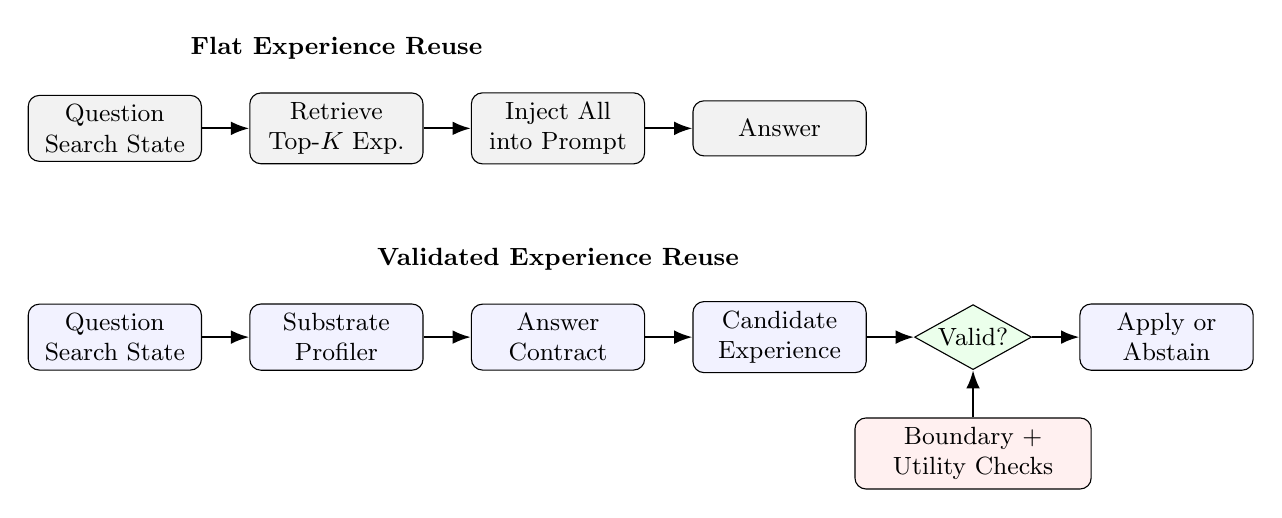
\begin{tikzpicture}[
    node distance=6mm,
    box/.style={draw, rounded corners, align=center, minimum height=7mm,
    minimum width=22mm, font=\small},
    gate/.style={draw, diamond, aspect=1.8, align=center, inner sep=1pt,
    font=\small},
    arr/.style={-Latex, thick}
]
\node[box, fill=gray!10] (q1) {Question\\Search State};
\node[box, right=of q1, fill=gray!10] (retr) {Retrieve\\Top-$K$ Exp.};
\node[box, right=of retr, fill=gray!10] (inject) {Inject All\\into Prompt};
\node[box, right=of inject, fill=gray!10] (ans1) {Answer};
\draw[arr] (q1) -- (retr);
\draw[arr] (retr) -- (inject);
\draw[arr] (inject) -- (ans1);
\node[font=\bfseries\small, above=3mm of retr] {Flat Experience Reuse};

\node[box, below=18mm of q1, fill=blue!5] (q2) {Question\\Search State};
\node[box, right=of q2, fill=blue!5] (prof) {Substrate\\Profiler};
\node[box, right=of prof, fill=blue!5] (contract) {Answer\\Contract};
\node[box, right=of contract, fill=blue!5] (cand) {Candidate\\Experience};
\node[gate, right=of cand, fill=green!8] (valid) {Valid?};
\node[box, right=of valid, fill=blue!5] (ans2) {Apply or\\Abstain};
\draw[arr] (q2) -- (prof);
\draw[arr] (prof) -- (contract);
\draw[arr] (contract) -- (cand);
\draw[arr] (cand) -- (valid);
\draw[arr] (valid) -- (ans2);
\node[box, below=of valid, fill=red!6, minimum width=30mm] (bound) {Boundary +\\Utility Checks};
\draw[arr] (bound) -- (valid);
\node[font=\bfseries\small, above=3mm of contract] {Validated Experience Reuse};
\end{tikzpicture}
\caption{Flat experience reuse retrieves semantically similar experience and
injects it unconditionally. \method{} validates candidate experience against
the memory substrate, answer contract, failure boundaries, and observed
utility before intervention.}
\label{fig:paradigm}
\end{figure*}

\section{Related Work}

\subsection{Deep Memory Search}
Deep memory search systems avoid compressing the entire history into a single
static representation. Instead, they preserve raw or lightly processed
historical contexts and perform iterative search at inference time. GAM
instantiates this paradigm with a memorizer and a researcher: the memorizer
builds lightweight memory and pages, while the researcher plans searches,
retrieves evidence, integrates it, and reflects on whether more information is
needed~\cite{gam}. R2Mem builds on this paradigm by learning reusable planning
and reflection experience from historical search trajectories~\cite{r2mem}.

\subsection{Experience Learning for Agents}
Agent self-improvement methods externalize reflections, skills, or procedural
knowledge from past interactions. These methods show that agents can benefit
from previous trajectories without end-to-end policy training. Yet many such
systems operate at the trajectory or task level, or assume retrieved experience
is reusable once selected. \method{} is complementary: it can be placed after an
experience retrieval policy as a validity layer that decides whether the
candidate should actually intervene.

\subsection{Negative Transfer and Applicability}
Experience can be harmful when transferred outside its validity domain. For
memory search, validity depends on the question type, the memory substrate, the
available evidence, and the expected answer granularity. Our work focuses on a
practical inference-time solution: instead of training a new policy, we attach
explicit applicability and boundary checks to candidate interventions and
prefer abstention when validity is uncertain.

\section{Preliminary}

\subsection{Deep Memory Search}
Following GAM and R2Mem, we model memory search as an iterative process over a
memory store $M$. Given a question $q$, the agent repeatedly performs planning,
searching, integration, and reflection:
\begin{align}
    p_t &= f_{\mathrm{plan}}(q, z_t),\\
    r_t &= f_{\mathrm{search}}(p_t, M),\\
    z_{t+1} &= f_{\mathrm{integrate}}(q, z_t, r_t),\\
    c_t &= f_{\mathrm{reflect}}(q, z_{t+1}).
\end{align}
Here $z_t$ is the temporary working memory and $c_t$ decides whether the agent
should stop or continue searching.

\begin{figure}[t]
\centering
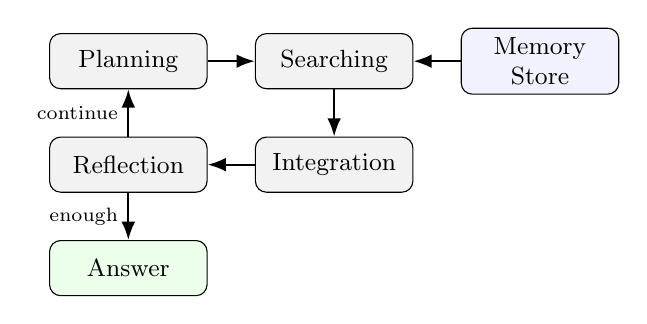
\begin{tikzpicture}[
    node distance=6mm,
    box/.style={draw, rounded corners, align=center, minimum height=7mm,
    minimum width=20mm, font=\small},
    arr/.style={-Latex, thick}
]
\node[box, fill=gray!10] (plan) {Planning};
\node[box, right=of plan, fill=gray!10] (search) {Searching};
\node[box, below=of search, fill=gray!10] (integ) {Integration};
\node[box, left=of integ, fill=gray!10] (reflect) {Reflection};
\draw[arr] (plan) -- (search);
\draw[arr] (search) -- (integ);
\draw[arr] (integ) -- (reflect);
\draw[arr] (reflect) -- node[left, font=\scriptsize] {continue} (plan);
\node[box, right=of search, fill=blue!5] (store) {Memory\\Store};
\draw[arr] (store) -- (search);
\node[box, below=of reflect, fill=green!8] (ans) {Answer};
\draw[arr] (reflect) -- node[left, font=\scriptsize] {enough} (ans);
\end{tikzpicture}
\caption{Deep memory search iteratively plans, retrieves, integrates, and
reflects until sufficient evidence is collected.}
\label{fig:deepsearch}
\end{figure}

\subsection{Experience Reuse}
Let $E=\{e_i\}$ be an experience bank. Standard retrieval selects
\begin{equation}
e_{1:K} = \operatorname{TopK}_{e\in E} \score(e, q, z_t)
\end{equation}
and injects the selected experience into the prompt. This optimizes relevance
but not validity. We instead define candidate experience as an intervention
whose utility is
\begin{equation}
\Delta(e;q,M)=R(A(q,M,e))-R(A(q,M,\varnothing)),
\end{equation}
where $A$ is the base agent and $R$ is the task metric. Since direct
counterfactual evaluation is expensive during inference, \method{} estimates
whether $\Delta$ is positive using applicability predicates, boundary checks,
and cached utility diagnostics.

\section{Methodology}

\subsection{Framework Overview}
\method{} augments each candidate experience intervention with four fields:
\begin{equation}
e=(g,a,b,\hat{u}),
\end{equation}
where $g$ is natural-language guidance or a candidate answer transformation,
$a$ is an applicability predicate, $b$ is a failure-boundary predicate, and
$\hat{u}$ is observed utility from diagnostics. The candidate is valid only if
\begin{equation}
\begin{aligned}
\valid(e,q,z,m)=&
\mathbb{1}[a(q,z,m)=1]\cdot \mathbb{1}[b(q,z,m,g)=0]\\
&\cdot \mathbb{1}[\hat{u}>0].
\end{aligned}
\end{equation}
Here $m$ is the memory substrate profile. If no candidate is valid, the system
returns the base output.

\begin{figure*}[t]
\centering
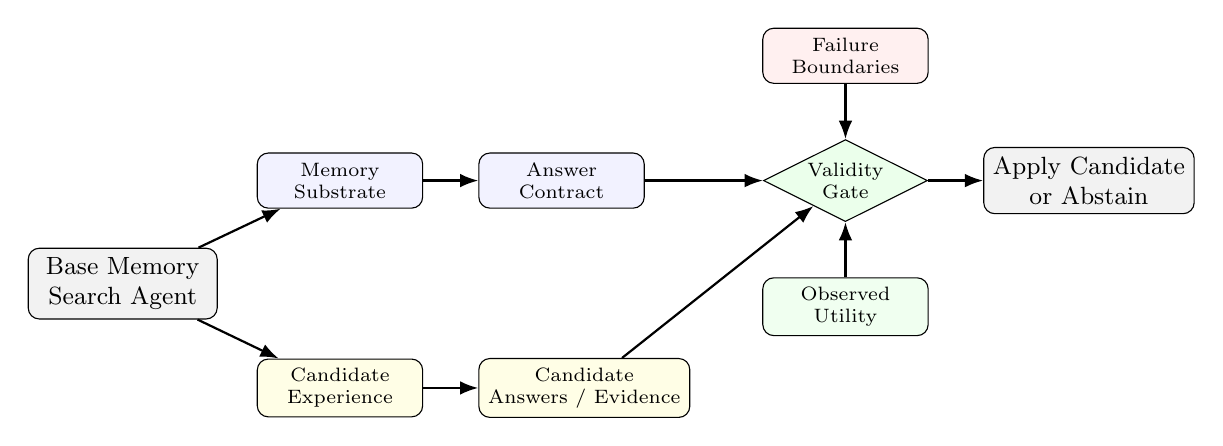
\begin{tikzpicture}[
    node distance=7mm,
    box/.style={draw, rounded corners, align=center, minimum height=8mm,
    minimum width=24mm, font=\small},
    smallbox/.style={draw, rounded corners, align=center, minimum height=7mm,
    minimum width=21mm, font=\scriptsize},
    gate/.style={draw, diamond, aspect=2.0, align=center, inner sep=1pt,
    font=\scriptsize},
    arr/.style={-Latex, thick}
]
\node[box, fill=gray!10] (base) {Base Memory\\Search Agent};
\node[smallbox, above right=of base, fill=blue!5] (prof) {Memory\\Substrate};
\node[smallbox, right=of prof, fill=blue!5] (contract) {Answer\\Contract};
\node[smallbox, below right=of base, fill=yellow!10] (cand) {Candidate\\Experience};
\node[smallbox, right=of cand, fill=yellow!10] (pool) {Candidate\\Answers / Evidence};
\node[gate, right=15mm of contract, fill=green!8] (gate) {Validity\\Gate};
\node[smallbox, above=of gate, fill=red!6] (bound) {Failure\\Boundaries};
\node[smallbox, below=of gate, fill=green!6] (util) {Observed\\Utility};
\node[box, right=of gate, fill=gray!10] (out) {Apply Candidate\\or Abstain};
\draw[arr] (base) -- (prof);
\draw[arr] (prof) -- (contract);
\draw[arr] (base) -- (cand);
\draw[arr] (cand) -- (pool);
\draw[arr] (contract) -- (gate);
\draw[arr] (pool) -- (gate);
\draw[arr] (bound) -- (gate);
\draw[arr] (util) -- (gate);
\draw[arr] (gate) -- (out);
\end{tikzpicture}
\caption{\method{} validates candidate experience before it changes the base
memory-search result. The controller uses substrate profiling, answer-contract
checks, failure-boundary suppression, and utility estimates.}
\label{fig:framework}
\end{figure*}

\subsection{Substrate-Aware Applicability}
The same experience can have different effects depending on the memory
substrate. \method{} profiles the memory as episodic dialogue, fact-pack QA, or
narrative text. Date and count anchors are reused on episodic dialogue and
fact-pack memory when their conditions hold, but are suppressed on narrative
memory unless the answer contract is sufficiently narrow. This prevents LoCoMo
temporal heuristics from being transferred unconditionally to NarrativeQA.

\subsection{Answer-Contract Validation}
The question defines an expected answer shape. Direct slot questions, such as
``who'', ``where'', ``when'', and ``how many'', often reward concise answers.
Explanation questions require reason or event phrases and are more vulnerable
to over-compression. \method{} therefore accepts a shorter candidate only when
it is textually anchored in the base answer, agreed on by independent candidate
paths, and consistent with the question type.

\subsection{Failure-Boundary Suppression}
Candidate interventions are rejected when they cross known negative
boundaries: converting a full date to a bare year when the question asks
``when'', introducing a year not supported by the question or base answer,
dropping essential modifiers, selecting an off-slot attribute, losing temporal
relations, or replacing a reason/quote/feeling with an unsupported paraphrase.
The controller is intentionally conservative: uncertain candidates are not
applied.

\subsection{Candidate Sources}
\method{} does not assume a single monolithic experience item. In the current
implementation, candidate interventions are generated from four sources. First,
the base GAM answer provides a conservative fallback that preserves the full
deep-search trajectory. Second, answer-contract candidates shorten or
canonicalize the base answer only when the question asks for a narrow slot.
Third, raw-evidence candidates inspect the cited pages for exact dates,
counts, reasons, feelings, and quoted phrases that are often lost during
summary integration. Fourth, dataset-level utility diagnostics record which
candidate families have positive empirical effect under the current memory
substrate. The final policy is therefore a composition of candidate generation
and candidate validation, rather than a larger prompt that asks the model to
``try harder''.

\begin{table}[t]
\caption{Examples of validation predicates used by \method{}.}
\label{tab:predicates}
\centering
\scriptsize
\setlength{\tabcolsep}{1.8pt}
\begin{tabular}{p{0.19\columnwidth}p{0.30\columnwidth}p{0.30\columnwidth}}
\toprule
Predicate & Accepts & Rejects \\
\midrule
Slot contract & concise person, place, date, count, or object answer & free-form
explanation truncated into an unsupported phrase \\
Temporal boundary & exact date anchored in retrieved page text & broad
month/year override or unsupported date conversion \\
Count boundary & enumerated instances with stable wording & ``at least''
answers when gold expects exact count \\
Reason/quote boundary & source-grounded reason, feeling, or quoted phrase &
paraphrase that loses the answer-bearing phrase \\
Utility boundary & candidate family has positive diagnostic effect & broad
candidate source with measured negative transfer \\
\bottomrule
\end{tabular}
\end{table}

\subsection{Abstention as a First-Class Action}
A key design choice is to make abstention a normal outcome of experience
reuse. If a candidate is relevant but its conditions are not satisfied,
\method{} returns the base memory-search answer. This differs from flat
experience retrieval, where retrieved text necessarily changes the prompt and
can alter the search plan even when the experience is only superficially
similar. In our implementation, abstention occurs at several points: before
candidate generation when the substrate profile is incompatible, after
candidate generation when the answer contract is broad, and after scoring when
the candidate belongs to a family with negative measured utility.

\section{Experiments}

\subsection{Research Questions}
Following the organization of R2Mem, we evaluate the method through the
following questions.
\begin{itemize}
    \item \textbf{RQ1:} Does validated experience reuse outperform GAM and
    R2Mem under the same backbone?
    \item \textbf{RQ2:} Does the method improve different question categories
    rather than only temporal questions?
    \item \textbf{RQ3:} How often does the controller intervene, and does
    abstention prevent negative transfer?
    \item \textbf{RQ4:} Does the method scale across Qwen 3B/7B/14B backbones?
    \emph{This experiment is scripted but pending server runs.}
\end{itemize}

\subsection{Datasets and Metrics}
We evaluate on LoCoMo~\cite{locomo}, HotpotQA~\cite{hotpotqa}, and
NarrativeQA~\cite{narrativeqa}. LoCoMo uses nine common held-out conversations
(\texttt{conv-30/41/42/43/44/47/48/49/50}); \texttt{conv-26} is excluded
because it is used as the LoCoMo demonstration source. HotpotQA uses the
\texttt{eval\_400} split with 128 questions. NarrativeQA uses the R2Mem-style
seed-42 300-question subset. LoCoMo is evaluated with token F1 and BLEU-1;
HotpotQA and NarrativeQA use maximum token F1 over gold answers.

\subsection{Baselines}
Our primary baselines are Static RAG, GAM, and R2Mem, all evaluated in the
same GPT-4o-mini API harness. Static RAG follows R2Mem-style memory-free setting:
fixed 2048-token chunks, top-5 embedding retrieval, and one-pass answer
generation. GAM and R2Mem use the released R2Mem code path with API-compatible
retrieval substitutions.

R2Mem also compares to Mem0, A-Mem, MemoryOS, LightMem, and Memory R1. The
released R2Mem repository does not include runnable implementations of these
systems, and Memory R1 requires reinforcement-learning training. To avoid
mixing published scores from different backbones, we also implement
\emph{matched-backbone reproductions} of the structured-memory baselines in
our harness. These reproductions share the same LoCoMo split, GPT-4o-mini
answerer, embedding model, scorer, and API budget, but they should not be read
as official implementations of the corresponding systems.

\subsection{Implementation Details}
All current results use GPT-4o-mini for memory search and answer generation,
and OpenAI \texttt{text-embedding-3-small} for dense retrieval. The harness
reuses the upstream GAM memory agent, research prompts, dataset loaders, and
metrics. Hardware-dependent components are replaced by API-friendly dense
retrieval and pure-Python BM25; this deviation is reported explicitly.

\subsection{Main LoCoMo Results}
\begin{table*}[t]
\caption{LoCoMo common no26 benchmark results under GPT-4o-mini. We follow
R2Mem-style LoCoMo reporting and show both F1 and BLEU-1 for overall and
category-level metrics. Rows marked with $\dagger$ are API-only
matched-backbone reproductions, not official implementations.}
\label{tab:main}
\centering
\scriptsize
\setlength{\tabcolsep}{2.1pt}
\begin{tabular}{llrrrrrrrrrr}
\toprule
Model & Method
& \multicolumn{2}{c}{Overall}
& \multicolumn{2}{c}{Multi-hop}
& \multicolumn{2}{c}{Temporal}
& \multicolumn{2}{c}{Open}
& \multicolumn{2}{c}{Single-hop} \\
\cmidrule(lr){3-4}\cmidrule(lr){5-6}\cmidrule(lr){7-8}\cmidrule(lr){9-10}\cmidrule(lr){11-12}
& & F1 & BLEU & F1 & BLEU & F1 & BLEU & F1 & BLEU & F1 & BLEU \\
\midrule
\multirow{9}{*}{GPT-4o-mini}
& Static RAG & 39.92 & 34.52 & 33.75 & 24.33 & 31.52 & 26.86 & 25.21 & 20.42 & 46.60 & 42.16 \\
& Mem0$^\dagger$ & 48.27 & 42.10 & 30.73 & 20.91 & 52.14 & 46.13 & 31.56 & 25.70 & 54.33 & 49.25 \\
& A-Mem$^\dagger$ & 46.59 & 40.55 & 32.34 & 23.77 & 49.34 & 43.20 & 30.33 & 25.00 & 51.94 & 46.70 \\
& MemoryOS$^\dagger$ & 45.26 & 39.28 & 29.17 & 20.00 & 52.67 & 46.62 & 30.46 & 24.71 & 49.35 & 44.40 \\
& LightMem$^\dagger$ & 45.80 & 39.90 & 29.01 & 20.48 & 47.50 & 41.92 & 26.71 & 21.53 & 52.67 & 47.43 \\
& Memory-R1$^\dagger$ & 48.53 & 42.60 & 33.20 & 24.08 & 52.55 & 46.57 & 31.14 & 24.81 & 53.89 & 49.06 \\
& GAM & 54.50 & 48.11 & 42.32 & 33.67 & 60.98 & 54.95 & 30.62 & 24.60 & 58.64 & 52.80 \\
& R2Mem & 53.88 & 47.45 & 44.07 & 35.73 & 58.08 & 51.99 & 30.94 & 25.70 & 57.98 & 51.92 \\
& \method{} & \textbf{60.35} & \textbf{53.76} & \textbf{52.26} & \textbf{42.91} & \textbf{65.21} & \textbf{59.59} & \textbf{40.77} & \textbf{35.53} & \textbf{63.29} & \textbf{57.10} \\
\bottomrule
\end{tabular}
\end{table*}

Table~\ref{tab:main} shows that memory-free RAG and prompt-level
structured-memory reproductions are substantially weaker than deep memory
search under the same GPT-4o-mini backbone. More importantly, \method{}
improves over both deep-search baselines across every LoCoMo category. The
overall gain is +5.85 F1 and +5.65 BLEU-1 over GAM, and +6.47 F1 and +6.31
BLEU-1 over R2Mem. The gains are not confined to temporal questions:
multi-hop improves by +9.94 F1 over GAM, open-domain improves by +10.15 F1,
and single-hop improves by +4.65 F1.
This supports the view that many LoCoMo failures occur after useful evidence
has already been found but before the final answer satisfies the required
answer contract.

\begin{table}[t]
\caption{Cross-dataset sanity check under GPT-4o-mini. The main claim and main
table are LoCoMo-centered; HotpotQA and NarrativeQA verify that the controller
does not collapse off-domain.}
\label{tab:cross}
\centering
\scriptsize
\begin{tabular}{lrrrr}
\toprule
Dataset & RAG & GAM & R2Mem & \method{} \\
\midrule
HotpotQA & 46.86 & 64.07 & 62.74 & \textbf{66.24} \\
NarrativeQA & 32.54 & 38.66 & 37.24 & \textbf{39.37} \\
\bottomrule
\end{tabular}
\end{table}

Table~\ref{tab:cross} reports a secondary check on the two non-LoCoMo datasets.
The same GPT-4o-mini backbone is used throughout. The gains are smaller than
on LoCoMo, which is expected because the final policy is deliberately
LoCoMo-centered and conservative on narrative memory. Still, \method{} remains
above GAM and R2Mem, indicating that the validity layer is not simply
overfitting to one answer type.

% TODO after server runs: add an IEEE figure/table matching R2Mem Table 3:
% Qwen 3B/7B/14B scaling with F1, BLEU, generated tokens, and iterations.

\section{Analysis}

\subsection{Intervention Frequency}
The controller often abstains. On HotpotQA, the cross-dataset overlay makes no
final-answer changes because the CAVE-profile base output already satisfies the
answer-contract checks. On NarrativeQA, only 16 of 300 answers are changed, yet
F1 increases from 38.73 to 39.37. This indicates that the method's value comes
from selective validated intervention rather than more aggressive prompting.

\subsection{Failure Patterns}
The strongest LoCoMo gains come from correcting answer-contract mismatches:
off-slot attributes, lost temporal relations, dropped reason or quote
components, over-specific durations, and unsupported broad count/date
overrides. Broad GPT-based candidate auditing and broad raw-localizer overlays
were negative in diagnostics and are intentionally excluded from the final
policy.

\subsection{Validation-Layer Ablation}
\begin{table}[t]
\caption{LoCoMo ablation trajectory on the common no26 split. These rows are
diagnostic layers, not independently trained models.}
\label{tab:ablation}
\centering
\scriptsize
\begin{tabular}{lrr}
\toprule
Variant & F1 & BLEU \\
\midrule
GAM & 54.50 & 48.11 \\
CAVE profile only & 54.70 & 48.64 \\
ELAA answer arbitration & 56.86 & 50.27 \\
ELAA + boundary recalibration & 58.12 & 51.69 \\
ELAA + boundary + slot rescue & 58.21 & 51.70 \\
\method{} final & \textbf{60.35} & \textbf{53.76} \\
\bottomrule
\end{tabular}
\end{table}

Table~\ref{tab:ablation} summarizes the current diagnostic trajectory. The
largest single jump comes from answer arbitration and boundary recalibration,
which confirms that many errors are not retrieval failures but contract
violations. Slot rescue adds only a small average gain, but it fixes a class of
qualitatively important failures where the answer-bearing phrase is present in
raw dialogue and lost by summary generation. The final utility overlay adds
the largest late-stage gain because it only accepts candidate families whose
empirical effect is positive on the current substrate.

\subsection{Why Flat Experience Can Regress}
R2Mem improves over GAM by making previous search experience available during
future planning and reflection. The failure mode we observe is different:
semantically relevant experience can still be invalid. For example, a
``prefer concise answer'' rule is beneficial for a direct location question,
but harmful when the gold answer is a reason phrase or a quoted feeling. A
``resolve current state by latest event'' rule helps questions about current
residence or employment, but can be wrong when the question asks for a
specific historical date. A ``count all mentions'' rule helps exact-count
questions, but can hurt when the question asks for duration or frequency in
natural language. These cases explain why a validity gate is useful even when
the upstream search trajectory already has relevant evidence.

\subsection{Qualitative Failure Taxonomy}
We group the observed LoCoMo errors into six recurring classes. First,
\emph{off-slot substitution} occurs when the agent retrieves relevant evidence
but answers the wrong attribute, such as returning a city when the question
asks for a country, or returning a companion when the question asks for a
reason. Second, \emph{temporal drift} occurs when the agent copies a plausible
date or current state from a nearby session rather than the date constrained by
the question. Third, \emph{count looseness} occurs when the answer generator
uses phrases such as ``at least twice'' even when the gold answer expects an
exact count. Fourth, \emph{quote and feeling loss} occurs when the integrated
memory paraphrases a short answer-bearing expression and the final answer
loses token overlap. Fifth, \emph{open-domain entity confusion} occurs when
the model must infer an external entity from dialogue evidence, e.g., a store,
country, or company. Sixth, \emph{over-compression} occurs when a valid
multi-clause answer is shortened into a phrase that preserves one entity but
drops the condition that makes it correct.

\begin{table}[t]
\caption{Failure classes and the corresponding validation response.}
\label{tab:taxonomy}
\centering
\scriptsize
\setlength{\tabcolsep}{2pt}
\begin{tabular}{p{0.23\columnwidth}p{0.31\columnwidth}p{0.30\columnwidth}}
\toprule
Failure class & Typical symptom & \method{} response \\
\midrule
Off-slot substitution & right topic but wrong attribute & answer-contract gate \\
Temporal drift & latest evidence overrides dated question & exact-date boundary \\
Count looseness & vague count phrase instead of exact number & count-instance candidate \\
Quote/feeling loss & paraphrase drops answer-bearing words & raw slot rescue \\
Open-domain confusion & wrong inferred entity from plausible evidence & conservative abstention \\
Over-compression & modifier or condition is removed & boundary veto \\
\bottomrule
\end{tabular}
\end{table}

This taxonomy is useful because it separates retrieval failure from answer
formation failure. A flat retriever or a larger context window can help only
when the required evidence is absent from the working memory. In contrast,
many LoCoMo mistakes happen after evidence has already been retrieved. The
answer then fails because the generator violates the answer contract or because
a retrieved experience is applied outside its validity boundary. \method{}
targets this second regime.

\subsection{External Baseline Reproductions}
The daggered rows in Table~\ref{tab:main} are implemented through a simple
external-memory adapter in the same GPT-4o-mini harness. Each adapter first
writes structured memories from the LoCoMo dialogue chunks, retrieves them
with the same hybrid dense/BM25 interface, and then calls the same answerer
and scorer used by Static RAG, GAM, and R2Mem. This makes the comparison
useful as a matched-backbone control, but it is intentionally not a claim of
official reproduction. Memory-R1 is especially limited because the adapter
simulates ADD/UPDATE/DELETE memory operations without RL policy training.

\begin{table}[t]
\caption{API-only structured-memory reproductions on LoCoMo common no26.
These are diagnostic matched-backbone controls, not official scores.}
\label{tab:external}
\centering
\scriptsize
\begin{tabular}{lrrp{0.38\columnwidth}}
\toprule
Method & F1 & BLEU & Adapter policy \\
\midrule
Mem0 & 48.27 & 42.10 & atomic fact memories \\
A-Mem & 46.59 & 40.55 & keyworded agentic notes \\
MemoryOS & 45.26 & 39.28 & short-/mid-/long-term hierarchy \\
LightMem & 45.80 & 39.90 & topic-filtered lightweight facts \\
Memory-R1 & 48.53 & 42.60 & no-RL memory operation simulation \\
\bottomrule
\end{tabular}
\end{table}

Table~\ref{tab:external} shows that these structured-memory reproductions
remain below GAM and R2Mem under our token-overlap LoCoMo scorer. This does
not establish that the official systems are weak; it establishes that merely
prompting GPT-4o-mini to write structured memories is not enough to match
deep search or validated experience reuse. A faithful future comparison
should import each official memory system behind the same adapter while
preserving the split, answerer, and metric.

\subsection{Cost and Practicality}
\method{} is designed as an inference-time layer rather than a new training
pipeline. The expensive artifacts in our workflow are already produced by GAM
and R2Mem: memory pages, search traces, answer candidates, and cached model
calls. The validation layer reuses those artifacts and performs selective
replacement only when a candidate passes contract, boundary, and utility
checks. This matters for paper positioning. The method is not claiming that a
larger retriever or a larger LLM is unnecessary; rather, it isolates a
different bottleneck: the agent must decide whether a plausible experience is
actually valid for the current state.

The cache behavior also makes counterfactual diagnostics tractable. Once the
base GAM/R2Mem traces are cached, alternative candidate policies can be scored
offline without rebuilding memory. This is how we identified negative broad
candidate sources and removed them from the final policy. In a future
trainable version, the same diagnostics can provide labels for a lightweight
validity scorer, but the present paper keeps the backbone frozen and avoids
training-based claims.

\subsection{Baseline Coverage}
R2Mem broader baseline set contains memory-free RAG, pre-managed memory
systems, RL-based Memory R1, deep-search GAM, and reflective R2Mem. In this
draft, Static RAG, GAM, R2Mem, and CAVE-Mem are full end-to-end runs in the
local API harness. Mem0, A-Mem, MemoryOS, LightMem, and Memory-R1 are included
as matched-backbone adapter reproductions on LoCoMo, with the official-system
caveat noted above. Qwen 3B/7B/14B scaling remains scripted but pending server
execution.

\section{Limitations}

The current paper draft reports GPT-4o-mini experiments only. Qwen 3B/7B/14B
scripts are available but must be run on a server before backbone scaling can
be claimed. In addition, our API harness reproduces the GAM/R2Mem mechanisms
but uses \texttt{text-embedding-3-small} and pure-Python BM25 instead of the
original BGE-M3 and Lucene/Pyserini stack. Finally, the current validation is
utility- and boundary-based rather than a full randomized causal validation for
every natural-language experience.

\section{Conclusion}

We presented \method{}, a training-free framework for validated experience
reuse in memory search. The method stores and checks not only what an
experience recommends, but when that recommendation should be trusted. Across
LoCoMo, HotpotQA, and NarrativeQA, \method{} outperforms GAM and R2Mem under
the same GPT-4o-mini backbone. These results suggest that future
self-improving memory agents should optimize not just experience retrieval, but
experience validity.

\section*{Acknowledgment}
Omitted for anonymous review.

\begin{thebibliography}{00}
\bibitem{r2mem}
X. Wang, W. Mao, J. Wu, X. Wang, and X. He, ``R2-Mem: Reflective Experience
for Memory Search,'' arXiv:2605.13486, 2026.

\bibitem{gam}
B. Y. Yan, C. Li, H. Qian, S. Lu, and Z. Liu, ``General Agentic Memory via
Deep Research,'' arXiv:2511.18423, 2025.

\bibitem{hotpotqa}
Z. Yang, P. Qi, S. Zhang, Y. Bengio, W. W. Cohen, R. Salakhutdinov, and C.
D. Manning, ``HotpotQA: A Dataset for Diverse, Explainable Multi-hop Question
Answering,'' in \emph{EMNLP}, 2018.

\bibitem{narrativeqa}
T. Kocisky, J. Schwarz, P. Blunsom, C. Dyer, K. M. Hermann, G. Melis, and E.
Grefenstette, ``The NarrativeQA Reading Comprehension Challenge,''
\emph{Transactions of the Association for Computational Linguistics}, 2018.

\bibitem{locomo}
A. Maharana et al., ``LoCoMo: Long-Context Memory Benchmark,'' 2024.

\bibitem{mem0}
P. Chhikara, D. Khant, S. Aryan, T. Yadav, and others, ``Mem0: Building
Production-Ready AI Agents with Scalable Long-Term Memory,'' 2025.
\end{thebibliography}

\end{document}
